
%% Use the first of the following lines during production to
%% easily spot "overfull boxes" in the output. Use the second
%% line for the final version.
%\documentclass[12pt,draft,letterpaper]{report}
\documentclass[12pt,letterpaper]{report}

% for debugging
%\usepackage{showframe}

% Fncychap is used for fancy chapter headings, but it also gives the formatting commands I needed to define the new 
% \appendixchapter command. You should look at its documentation and pick a nice style to use.
\usepackage{fncychap}
\sloppy

% Appendix allows the inclusion of a line for "appendices", which otherwise won't get the right page number. You must
% use the [toc] option.
\usepackage[toc]{appendix}

% Tocloft is used to create the new list of appendices. You must use the [titles] option.
\usepackage[titles]{tocloft}

% Number the subsubsections and include them in the TOC
\setcounter{secnumdepth}{3}
\setcounter{tocdepth}{3}

% Create list of appendices, and don't include appendices in the table of contents
\newlistof{appendixchapter}{apx}{List of Appendices}

\newcommand{\appendixchapter}[1]{%
    \refstepcounter{appendixchapter}%
    \refstepcounter{chapter}%
    \renewcommand{\DOTIS}[1]{\DOCH \DOTI{#1}}
    \chapter*{#1}
    \addcontentsline{apx}{appendixchapter}{Appendix \protect\numberline{\theappendixchapter}#1}\par%
    \vspace {-1.47cm}}
    
\renewcommand{\theappendixchapter}{\Alph{appendixchapter}}

\newcommand{\appendixsection}[1]{%
    \refstepcounter{section}%
    \section*{\protect{\thesection}\hspace{2.6ex}#1}}
    
\newcommand{\appendixsubsection}[1]{%
    \refstepcounter{subsection}%
    \subsection*{\protect{\thesubsection}\hspace{2.5ex}#1}}


%% Replace the title, name, advisor name, graduation date and dedication below with
%% your own. Graduation months must be January, May or September.
\newcommand{\thesistitle}{Unsupervised Deep Learning}
\newcommand{\thesisauthor}{Rostislav Goroshin}
\newcommand{\thesisadvisor}{Professor Yann LeCun}
\newcommand{\graddate}{September 2015}

\renewcommand*\contentsname{Table of Contents}

%% The following makes chapters and sections, but not subsections,
%% appear in the TOC (table of contents). Increase to 2 or 3 to
%% make subsections or subsubsections appear, respectively. It seems
%% to be usual to use the "1" setting, however.
\setcounter{tocdepth}{1}

%% Sectional units up to subsubsections are numbered. To number
%% subsections, but not subsubsections, decrease this counter to 2.
\setcounter{secnumdepth}{3}

%% Page layout (customized to letter paper and NYU requirements):
\setlength{\oddsidemargin}{.6in}
\setlength{\textwidth}{5.8in}
\setlength{\topmargin}{.1in}
\setlength{\headheight}{0in}
\setlength{\headsep}{0in}
\setlength{\textheight}{8.3in}
\setlength{\footskip}{.5in}

%% Use the following commands, if desired, during production.
%% Comment them out for final version.
%\usepackage{layout} % defines the \layout command, see below
%\setlength{\hoffset}{-.75in} % creates a large right margin for notes and \showlabels

%% Controls spacing between lines (\doublespacing, \onehalfspacing, etc.):
\usepackage{setspace}

%% Allows me to rotate anything

%% Use the line below for official NYU version, which requires
%% double line spacing. For all other uses, this is unnecessary,
%% so the line can be commented out.
\doublespacing % requires package setspace, invoked above

%% Each of the following lines defines the \com command, which produces
%% a comment (notes for yourself, for instance) in the output file.
%% Example:    \com{this will appear as a comment in the output}
%% Choose (uncomment) only one of the three forms:
%\newcommand{\com}[1]{[/// {#1} ///]}       % between [/// and ///].
\newcommand{\com}[1]{\marginpar{\tiny #1}} % as (tiny) margin notes
%\newcommand{\com}[1]{}                     % suppress all comments.

%% This inputs your auxiliary file with \usepackage's and \newcommand's:
%% It is assumed that that file is called "definitions.tex".
% !TEX root = thesis.tex

% Graphics:
\usepackage[final]{graphicx}
\usepackage{afterpage}
%\usepackage{graphicx} % use this line instead of the above to suppress graphics in draft copies
%\usepackage{graphpap} % \defines the \graphpaper command

% Indent first line of each section:
\usepackage{indentfirst}

% Good AMS stuff:
\usepackage{amsthm} % facilities for theorem-like environments
\usepackage[tbtags]{amsmath} % a lot of good stuff!

% Fonts and symbols:

\usepackage{amsfonts}
\usepackage{amssymb}
\usepackage{array}
\usepackage{txfonts}
\usepackage{graphicx}
\usepackage{caption}
\usepackage{subcaption}
\usepackage{mdwlist}
\usepackage{graphics}
\usepackage{rotating}
\usepackage{pdfpages}
\usepackage{fancyvrb}
\usepackage{booktabs}
\usepackage{tabularx}
\usepackage{multirow}
\usepackage{verbatim}
\usepackage{algorithm}
\usepackage{algorithmic}
%\usepackage[backend=biber, style=numeric, maxnames=99, backref=false]{biblatex}
\usepackage[style=numeric, maxnames=99, backref=false]{biblatex}

% Added by me (Jonathan):
%\usepackage{adjustbox}
%\usepackage{xfrac}
%\usepackage[font=small]{subcaption}
%\usepackage[hidelinks]{hyperref}
%\usepackage{nicefrac}
%\usepackage{tabularx}
\usepackage{placeins}

\setlength{\bibitemsep}{\baselineskip}
\bibliographystyle{plain}%Choose a bibliograhpic style
\bibliography{references}

\renewcommand{\le}{\leqslant}
\renewcommand{\ge}{\geqslant}
\renewcommand{\emptyset}{\ensuremath{\varnothing}}
\newcommand{\ds}{\displaystyle}
\newcommand{\R}{\ensuremath{\mathbb{R}}}
\newcommand{\Q}{\ensuremath{\mathbb{Q}}}
\newcommand{\Z}{\ensuremath{\mathbb{Z}}}
\newcommand{\N}{\ensuremath{\mathbb{N}}}
\newcommand{\T}{\ensuremath{\mathbb{T}}}
\newcommand{\fix}{\marginpar{FIX}}
\newcommand{\new}{\marginpar{NEW}}
\newcommand{\dx}{\mathrm{d}x}
\newcommand{\dy}{\mathrm{d}y}
\newcommand{\df}{\mathrm{d}f}
\newcommand{\dv}{\mathrm{d}v}
\newcommand{\eps}{\varepsilon}
\newcommand{\closure}[1]{\ensuremath{\overline{#1}}}
\DeclareMathOperator*{\argmax}{arg\,max}

\long\def\tbl#1#2
{
 \setbox\tempbox\hbox{\tablefont #2}%
 \tabledim\hsize\advance\tabledim by -\wd\tempbox
 \tempdimen\wd\tempbox
	\global\divide\tabledim\tw@
 \caption{#1}
	\centerline{\box\tempbox}
}

%\setlength{\intextsep}{0.6\baselineskip}
%\setlength{\belowcaptionskip}{-1ex} % remove extra space above and below in-line float
%\setlength{\belowcaptionskip}{-0.5\baselineskip} \addtolength{\belowcaptionskip}{1.5ex}
\setlength{\intextsep}{3ex plus 2pt minus 2pt}


%% Cross-referencing utilities. Use one or the other--whichever you prefer--
%% but comment out both lines for final version.
%\usepackage{showlabels}
%\usepackage{showkeys}

\begin{document}
%% Produces a test "layout" page, for "debugging" purposes only.
%% Comment out for final version.
%\layout % requires package layout (see above, on this same file)

%%%%%% Title page %%%%%%%%%%%
%% Sets page numbering to "roman style" i, ii, iii, iv, etc:
\pagenumbering{roman}
%
%% No numbering in the title page:
\thispagestyle{empty}
%
\begin{center}
  {\Large\textbf{\thesistitle}}
  \vspace{.7in}

  by
  \vspace{.7in}

  \thesisauthor
  \vfill

\begin{doublespace}
  A dissertation submitted in partial fulfillment\\
  of the requirements for the degree of\\
  Doctor of Philosophy\\
  Department of Computer Science\\
  New York University\\
  \graddate
\end{doublespace}
\end{center}
\vfill

\noindent\makebox[\textwidth]{\hfill\makebox[2.5in]{\hrulefill}}\\
\makebox[\textwidth]{\hfill\makebox[2.5in]{\hfill\thesisadvisor\hfill}}
\newpage
%%%%%%%%%%%%% Optional Blank page %%%%%%%%%%%%%%%%%%
%\thispagestyle{empty}
%\vspace*{0in}
%This page intentionally left blank.
%\newpage

%%%%%%%%%%%%%% Dedication %%%%%%%%%%%%%%%%%
%% Comment out the following lines if you do not want to dedicate
%% this to anyone...
\begin{center}
\section*{Dedication}\addcontentsline{toc}{section}{Dedication}
\end{center}
Parents and friends
\newpage
%%%%%%%%%%%%%% Acknowledgements %%%%%%%%%%%%
%% Comment out the following lines if you do not want to acknowledge
%% anyone's help...
\section*{Acknowledgements}\addcontentsline{toc}{section}{Acknowledgements}
%Firstly, I would like to thank my advisor Yann LeCun for believing in
unsupervised learning both for machines and students. His unwaivering
enthusiasm and commitment to tackling the hard problems inspired many to make
steady progress in this emerging area of research.

I thank many colleagues that have passed through our lab over the years.
Particularly, Joan Bruna who tough me that patient, deliberate thought is the
surest way to find structure in chaos.  I thank Jonathan Tompson for being a
great friend and showing me what it means to be a truly great
multi-disciplinary engineer.  I owe a debt of gratitude to David Eigen, who
provided invaluable insight to many hard problems. My thanks to the
neuroscience folks ``across the street'', Eero Simoncelli and his lab members,
for providing many insightful discussions. Many thanks to Julian Panetta for
his patient help in everything from proof-reading papers to answering many
``embarrassing'' computer science related questions.  
      
I'm thankful to my old friends Mohammad and Ramzy for providing their
friendship, guidance, support, and encouragement over many years.  
Thanks to my friend William from Georgia Tech for always being available for a chat.  
I thank my friends and colleagues at NSWC-PCD for their many years of support and
encouragement. Finally, I'm grateful to my parents who have remained patient
and supportive through my many years in school.  Last, but certainly not least,
thank you Emer for your loving support.  

 

\newpage
%%%% Abstract %%%%%%%%%%%%%%%%%%
\section*{Abstract}\addcontentsline{toc}{section}{Abstract}
%Much of computer vision has been devoted to the question of representation
through feature extraction. Useful features transform the raw pixel intensity
values to a representation in which common problems such as identification,
tracking, and segmentation of objects are easier to solve. Recently, deep
feature hierarchies have proven to be immensely successful at solving many
problems in computer vision. In the supervised setting, these hierarchies are
trained to solve specific problems by minimizing an objective function of the
data and problem specific label information. Recent findings suggest that
despite being trained on a specific task, the learned features can be
transferred across multiple visual tasks. These findings suggests that there
exists a generically useful feature representation for natural visual data.    

This work aims to uncover the principles that lead to these generic feature
representations in the unsupervised setting that doesn't resort to problem
specific label information. We begin by reviewing relevant prior work,
particularly the literature on auto-encoder networks and energy based learning.
We introduce a new regularizer for auto-encoders which plays an analogous role
to the partition function in probabilistic graphical models.  Next we explore
the role of specialized encoder architectures for sparse inference. The
remainder of the thesis explores visual feature learning from video. We
establish a connection between slow-feature learning and metric learning, and
experimentally demonstrate that semantically coherent metrics can be learned
from natural videos. Finally, we posit that useful features linearize
natural image transformations in video. To this end, we introduce a new
architecture and loss for training deep feature hierarchies that linearize the
transformations observed in unlabeled natural video sequences by learning to
predict future frames in the presence of uncertainty.           


 

\newpage
%%%% Table of Contents %%%%%%%%%%%%
\tableofcontents
%%%%% List of Figures %%%%%%%%%%%%%
%% Comment out the following two lines if your thesis does not
%% contain any figures. The list of figures contains only
%% those figures included withing the "figure" environment.
\cleardoublepage
\addcontentsline{toc}{section}{List of Figures}
\listoffigures
\newpage

%%%%% List of Tables %%%%%%%%%%%%%
%% Comment out the following two lines if your thesis does not
%% contain any tables. The list of tables contains only
%% those tables included withing the "table" environment.
\listoftables\addcontentsline{toc}{section}{List of Tables}
\newpage

%\listofappendixchapter\addcontentsline{toc}{section}{List of Appendices}
%\newpage

%%%%% Body of thesis starts %%%%%%%%%%%%
\pagenumbering{arabic} % switches page numbering to arabic: 1, 2, 3, etc.
%% Introduction. If your thesis has no introduction, or chapter 1 is
%% meant to be the introduction, then comment out the lines below.
%\section*{Introduction}\addcontentsline{toc}{chapter}{Introduction}
\chapter{Introduction} 
\label{chaper:introduction} 
%%Tracking of human bodies in images is a long standing problem in computer vision research, with a history of prior art beginning as early as the 1970s~\cite{Fischler73, hogg1983model}. The wide variety of important applications that rely on accurate and stable estimates of human pose has been a strong motivator for much of this research. Perhaps chief among these applications has been motion capture for the entertainment industry, where human body localization and pose inference enables accurate reconstruction and re-targeting of animation data to synthetic computer generated models. It is therefore not surprising that a large portion of the literature relates to \emph{marker-based} motion capture, with a specific focus on capturing realistic skeletal animation data. Furthermore, many commercial solutions exist for \emph{marker-based} motion capture, such as those from Vicon and Optitrack, which are able to predict marker location within sub-millimeter accuracy and at very high frame-rates (up to a few thousand hertz).

However, there are many applications that require accurate tracking of humans in images without the use of adding visual annotations or markers. Human-Computer-Interaction (HCI), virtual reality, surveillance, gait analysis, medical diagnosis applications, biometrics, action recognition and many other applications are examples where existing \emph{marker-based} motion capture solutions are often inappropriate or infeasible. Furthermore, recent applications in HCI demand real-time performance which has proven to be a particularly difficult constraint, especially for solutions using only RGB-based capture devices. Targeting real-time and low-cost applications for human pose estimation, this work focuses on human body localization without the use of visual annotations - so called \emph{marker-less} motion capture. Furthermore, this thesis explores solutions of the localization problem that make use of only one camera view (or monocular capture) as this is the lowest barrier of entry for wide-spread use. While calibrated multi-camera capture rigs are feasible for off-line applications, the ubiquity of single RGB and depth cameras (in devices such as laptops and cell phones) make this input modality an appealing research framework.

\begin{figure}[ht]
\centering
	\subcaptionbox{\footnotesize Shape \& Clothing Variation\label{fig:difficult_a}}{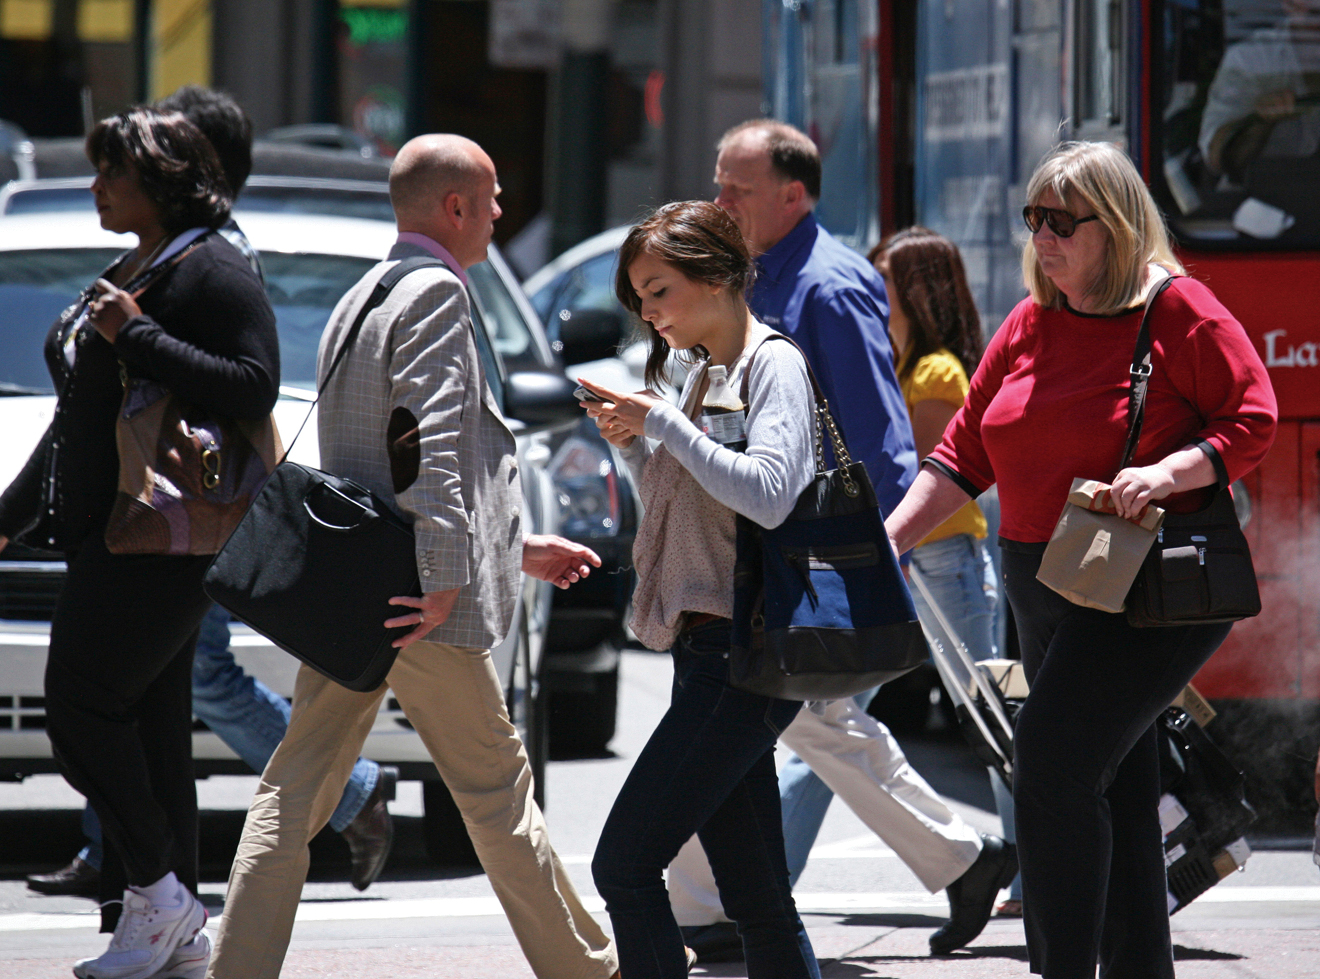
\includegraphics[height=3.9cm]{figures_introduction/pedestrian}}
	\subcaptionbox{\footnotesize Lighting Variation\label{fig:difficult_b}}{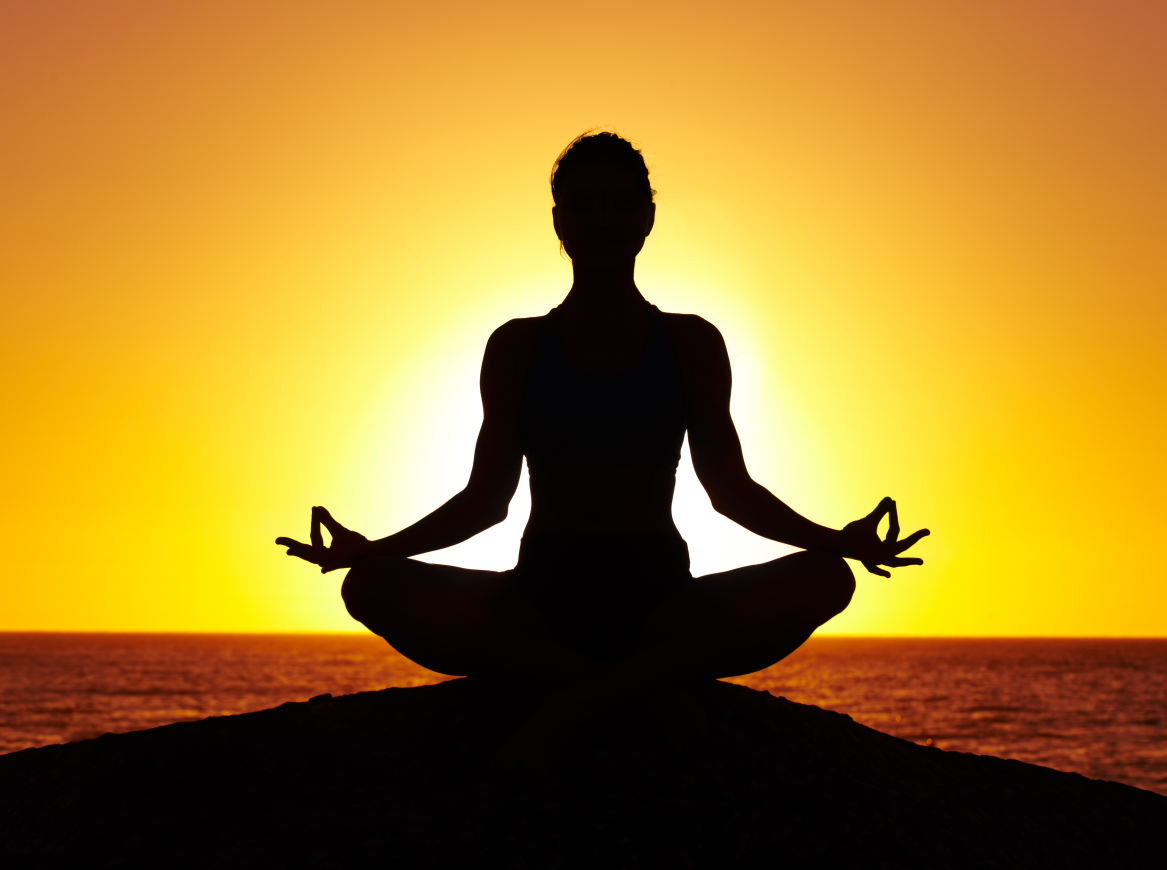
\includegraphics[trim=1.7cm 1.0cm 1.5cm 0.5cm, clip=true, height=3.9cm]{figures_introduction/yoga-pose}}
	\subcaptionbox{\footnotesize Self Occlusion\label{fig:difficult_c}}{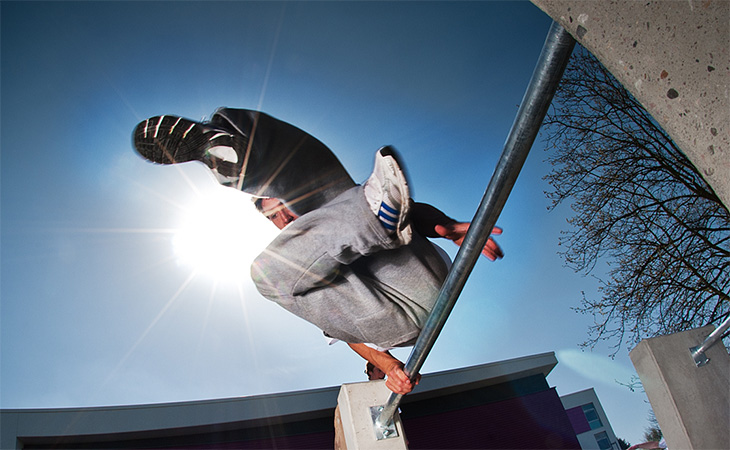
\includegraphics[trim=3.0cm 0.0cm 6.5cm 2.0cm, clip=true, height=3.9cm]{figures_introduction/x-move_parkour_.jpg}}
        \caption{Difficult Samples for Human Body Pose Recognition}
        \label{fig:difficult}
\end{figure}

Human body localization is complicated and difficult for numerous reasons, and some difficult examples are shown in Figure~\ref{fig:difficult}. As with many computer vision applications, the high dimensional nature of the image input makes inferring the low-dimensional pose representation difficult since the input dimensionality cannot be easily enumerated. However, unlike many classic computer vision tasks, human body tracking also involves localizing body parts that undergo large amounts of deformation and exhibit wide variation in both body-shape and appearance. Deformation increases the intrinsic input dimensionality of the space of possible poses and furthermore leads to occlusion, which means that pose inference must be performed with potentially missing data. Appearance variation can be the result of clothing, lighting variation or the subjects age or gender; therefore any inference solution must learn invariance in order to provide a stable estimate of pose under such wildly varying conditions. Lastly, large and comprehensive datasets exist for image classification tasks~\cite{deng2009imagenet}, however human-body pose datasets are many orders of magnitude smaller~\cite{modec,andriluka14cvpr,Johnson10}. The lack of a comprehensive standard dataset has traditionally made training robust discriminative architectures difficult as such networks are prone to over-training when the training set sizes are limited.

Despite these significant challenges, this work will present a framework for human body pose localization that offers a significant improvement over existing traditional architectures. The basis for all the tracking solutions presented in this thesis is the use of Convolutional Networks (ConvNets), which have seen a recent surge in success and popularity due to advances in Graphics Processing Unit (GPU) hardware as well as new and improved techniques for training them. ConvNets are biologically inspired variants of multi-layered perceptrons, which exploit spatial correlation in natural images by extracting features generated by localized convolution kernels. In the context of object detection, the use of fully convolutional networks result in trained detectors which are invariant to translation, and this work makes heavy use of this feature for the architectures presented in Parts \ref{part:two}, \ref{part:three} and \ref{part:four}. A full-review of ConvNets - specifically their formulation and training via the Back-Propagation algorithm - is outside the scope of this thesis and interested readers should refer to \cite{reading_list} for an overview of seminal literature.

ConvNets have been used successfully to solve many difficult machine learning problems: image classification~\cite{pedestrianCVPR13, overfeatSermanet, ImageNet_NIPS2012_0534, googlenet}, scene understanding~\cite{Farabet}, video analysis~\cite{KarpathyCVPR14} and natural language processing~\cite{ilya_sequence,cho_emnlp_2014}. Likewise, they have recently out-performed all existing models on the task of hand-pose recognition~\cite{tompsonTOG14} using an depth camera source, and monocular human-body pose recognition using an RGB camera~\cite{tompsonnips2014, arjunaccv2014, jainiclr2014, deeppose, chennips2014, tompson_efficient}. In this work, we will present our results for the current state-of-the-art models (at time of writing) for human body and hand pose recognition.

\subsection*{Thesis Outline}

This thesis will explore solutions to two difficult computer vision problems related to the localization of humans in images: 1) monocular hand-pose recognition from depth images and 2) monocular full body-pose recognition from RGB images. This exploration will cover four primary publications \cite{tompsonTOG14}, \cite{tompsonnips2014}, \cite{arjunaccv2014}, \cite{tompson_efficient} in Parts \ref{part:one}, \ref{part:two}, \ref{part:three} and \ref{part:four} respectively. Within each part, the first section will define the specific problem and present an overview of the architecture. The second section will present the model and any algorithmic details necessary to repeat experiments. Then the final solution will present experimental results, compare our work with previous state-of-the-art and describe any limitations.

\subsection*{Summary of Contributions}

The following is a summary of the major contributions of this thesis:

\begin{itemize}

\item In Part~\ref{part:one} we describe a novel pipeline for both offline ground truth dataset creation, as well as real-time pose-detection of human hands in depth video. While Neural Networks have been used for pose detection of a limited set of discrete hand gestures (for instance discriminating between a closed fist and an open palm)~\cite{nagi,nowlan}, to our knowledge this is the first work that has attempted to use such networks to perform dense feature extraction of human hands in order to infer continuous pose.

\item In Part~\ref{part:two} we describe a novel ConvNet architecture which combines a traditional sliding-window based part detector with a Graphical Model. We describe a graphical model formulation which is inspired by standard MRF belief propagation, which can be trained jointly with a standard deep-learning architecture to improve detection performance. At the time of writing, this model is the state-of-the-art model for the FLIC~\cite{modec}, LSP~\cite{Johnson10} and MPII~\cite{andriluka14cvpr} datasets.

\item In Part~\ref{part:three} we show that simple motion features can be used to significantly improve the performance of traditional ConvNet architectures. To our knowledge, this was the first work to empirically examine the impact of multi-frame inputs to ConvNets in the application of pose detection.

\item In Part~\ref{part:four} we examine the issue of localization accuracy degradation in ConvNet architecture due to spatial-pooling layers. We present a novel cascaded architecture, that makes use of shared features, in order to improve localization accuracy while maintaining runtime performance. We are the first to show that a ConvNet trained to infer the 2D pose of humans in images is able to be competitive with - and in some cases out-perform - humans trained on the same task.

\end{itemize}
\chapter{Related Work}
\label{chapter:related_work}
\chapter{Saturating Auto-Encoders}
\label{chapter:SATAE}
\section{Introduction} 
This Chapter introduces a new latent state regularization method for auto-encoders. 
We show that the saturation regularizer explicitly limits the auto-encoder's capacity to
reconstruct inputs which are not near the data manifold. Connections are established with 
other auto-encoder regularization methods, as well as with the partition function in 
probabilistic models. 

When minimizing reconstruction loss alone, the standard auto-encoder
does not typically learn any meaningful hidden representation of the data. Well
known theoretical and experimental results show that a linear auto-encoder with
trainable encoding and decoding matrices, $W^e$ and $W^d$ respectively, learns
the identity function if $W^e$ and $W^d$ are full rank or over-complete. The
linear auto-encoder learns the principle variance directions (PCA) if $W^e$ and
$W^d$ are rank deficient \cite{DHS}. It has been observed that other
representations can be obtained by regularizing the latent representation. This
approach is exemplified by the Contractive and Sparse Auto-Encoders \cite{CAE}
\cite{SAE1} \cite{SAE2}. Intuitively, an auto-encoder with limited capacity
will focus its resources on reconstructing portions of the input space in which
data samples occur most frequently. From an energy based perspective,
auto-encoders achieve low reconstruction cost in portions of the input space
with high data density (recently, \cite{bengio_new} has examined this
perspective in depth). If the data occupies some low dimensional manifold in
the higher dimensional input space then minimizing reconstruction error
achieves low energy on this manifold. Useful latent state regularizers raise
the energy of points that do not lie on the manifold, thus playing an analogous
role to minimizing the partition function in maximum likelihood models. In this
work we introduce a new type of regularizer that does this explicitly for
auto-encoders with a non-linearity that contains at least one flat (zero
gradient) region. We show examples where this regularizer and the choice of
nonlinearity determine the feature set that is learned by the auto-encoder.      

\section{Latent State Regularization}  Several auto-encoder variants which
regularize their latent states have been proposed, they include the sparse
auto-encoder and the contractive auto-encoder\cite{SAE1}\cite{SAE2}\cite{CAE}.
The sparse auto-encoder includes an over-complete basis in the encoder and
imposes a sparsity inducing (usually $L_1$) penalty on the hidden activations.
This penalty prevents the auto-encoder from learning to reconstruct all
possible points in the input space and focuses the expressive power of the
auto-encoder on representing the data-manifold. Similarly, the contractive
auto-encoder avoids trivial solutions by introducing an auxiliary penalty which
measures the square  Frobenius norm of the Jacobian of the latent
representation with respect to the inputs. This encourages a constant latent
representation except around training samples where it is counteracted by the
reconstruction term. It has been noted in \cite{CAE} that these two approaches
are strongly related. The contractive auto-encoder explicitly encourages small
entries in the Jacobian, whereas the sparse auto-encoder is encouraged to
produce mostly zero (sparse) activations which can be designed to correspond to
mostly flat regions of the nonlinearity, thus also yielding small entries in
the Jacobian.

\subsection{Saturating Auto-Encoder through Complementary Nonlinearities}
Our goal is to introduce a simple new regularizer which explicitly raises
reconstruction error for inputs not near the data manifold. Consider activation
functions with at least one flat region; these include shrink, rectified
linear, and saturated linear (Figure~\ref{fig:nonlin}). Auto-encoders with such
nonlinearities lose their ability to accurately reconstruct inputs which
produce activations in the zero-gradient regions of their activation functions.
Let us denote the auto-encoding function $x_r = G(x,W)$, $x$ being the input,
$W$ the trainable parameters in the auto-encoder, and $x_r$ the reconstruction.
One can define an energy surface through the reconstruction error: \[ E_W(x) =
||x-G(x,W)||^2 \] Let's imagine that $G$ has been trained to produce a low
reconstruction error at a particular data point $x^*$. If $G$ is constant when
$x$ varies along a particular direction $v$, then the energy will grow
quadratically along that particular direction as $x$ moves away from $x^*$. If
$G$ is trained to produce low reconstruction errors on a set of samples while
being subject to a regularizer that tries to make it constant in as many
directions as possible, then the reconstruction energy will act as a {\em
contrast function} that will take low values around areas of high data density
and larger values everywhere else (similarly to a negative log likelihood
function for a density estimator).

The proposed auto-encoder is a simple implementation of this idea.  Using the
notation $W =\{W^e,B^e,W^d,B^d\}$, the auto-encoder function is defined as \[
G(x,W) = W^d F(W^e x+B^e) + B^d \] where $W^e$, $B^e$, $W^d$, and $B^d$ are the
encoding matrix, encoding bias, decoding matrix, and decoding bias,
respectively, and $F$ is the vector function that applies the scalar function
$f$ to each of its components. $f$ will be designed to have "flat spots", i.e.
regions where the derivative is zero (also referred to as the saturation
region).

The loss function minimized by training is the sum of the reconstruction energy
$E_W(x)=||x-G(x,W)||^2$ and a term that pushes the components of $W^e x + B^e$
towards the flat spots of $f$. This is performed through the use of a {\em
complementary function} $f_c$, associated with the non-linearity $f(z)$. The
basic idea is to design $f_c(z)$ so that its value corresponds to the distance
of $z$ to one of the flat spots of $f(z)$. Minimizing $f_c(z)$ will push $z$
towards the flat spots of $f(z)$. With this in mind, we introduce a penalty of
the form $f_c(\sum_{j=1}^d W^e_{ij}x_j + b^e_i)$ which encourages the argument
to be in the saturation regime of the activation function ($f$). We refer to
auto-encoders which include this regularizer as Saturating Auto-Encoders
(SATAEs). For activation functions with zero-gradient regime(s) the
complementary nonlinearity ($f_c$) can be defined as the distance to the
nearest saturation region. Specifically, let $S = \{z \mid  f'(z) = 0\}$ then
we define $f_c(z)$ as: 

\begin{equation} f_c(z) = \inf_ {z' \in S} |z-z'|.   \end{equation}   

\begin{figure} \centering 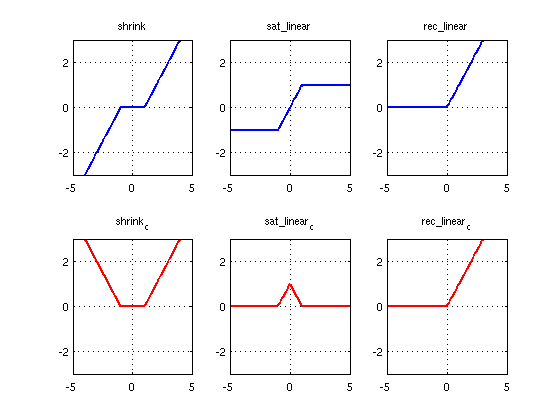
\includegraphics[scale=0.6]{./figures/SATAE/compliments.png}
\caption{Three nonlinearities (top) with their associated complementary
regularization functions(bottom).}  \label{fig:nonlin} \end{figure} 

\noindent Figure 1 shows three activation functions and their associated
complementary nonlinearities. The complete loss to be minimized by a SATAE with
nonlinearity $f$ is: 

\begin{equation} L = \sum_{x \in D} \frac{1}{2} \|x-\left(W^d F(W^e
x+B^e)+B^d\right)\|^2 + \alpha \sum_{i=1}^{d_h}f_c(W^e_i x + b^e_i),
\end{equation}    

\noindent where $d_h$ denotes the number of hidden units. The hyper-parameter
$\alpha$ regulates the trade-off between reconstruction and saturation.  

\section{Effect of the Saturation Regularizer} We will examine the effect of
the saturation regularizer on auto-encoders with a variety of activation
functions. It will be shown that the choice of activation function is a
significant factor in determining the type of basis the SATAE learns. First, we
will present results on toy data in two dimensions followed by results on
higher dimensional image data.

\subsection{Visualizing the Energy Landscape}  Given a trained auto-encoder the
reconstruction error can be evaluated for a given input $x$. For
low-dimensional spaces ($\mathbb{R}^n$, where $n \leq 3$) we can evaluate the
reconstruction error on a regular grid in order to visualize the portions of
the space which are well represented by the auto-encoder. More specifically we
can compute $E(x) = \frac{1}{2} \|x - x_r \|^2$ for all $x$ within some bounded
region of the input space. Ideally, the reconstruction energy will be low for
all $x$ which are in the training set and high elsewhere.
Figures~\ref{fig:toyshrink} and~\ref{fig:toysatlinear} depict the resulting
reconstruction energy for inputs $x \in \mathbb{R}^2$, and  $-1 \leq x_i \leq
1$. Black corresponds to low reconstruction energy. The training data consists
of a one dimensional manifold shown overlain in yellow.
Figure~\ref{fig:toyshrink} shows a toy example for a SATAE which uses ten basis
vectors and a shrink activation function. Note that adding the saturation
regularizer decreases the volume of the space which is well reconstructed,
however good reconstruction is maintained on or near the training data
manifold. The auto-encoder in Figure~\ref{fig:toysatlinear} contains two
encoding basis vectors (red), two decoding basis vectors (green), and uses a
saturated-linear activation function. The encoding and decoding bases are
unconstrained. The unregularized auto-encoder learns an orthogonal basis with a
random orientation. The region of the space which is well reconstructed
corresponds to the outer product of the linear regions of two activation
functions; beyond that the error increases quadratically with the distance.
Including the saturation regularizer induces the auto-encoder basis to align
with the data and to operate in the saturation regime at the extreme points of
the training data, which limits the space which is well reconstructed. Note
that because the encoding and decoding weights are separate and unrestricted,
the encoding weights were scaled up to effectively reduce the width of the
linear regime of the nonlinearity. 

\subsection{SATAE-shrink} Consider a SATAE with a shrink activation function
and shrink parameter $\lambda$. The corresponding complementary nonlinearity,
derived using Equation 1 is given by: \begin{equation} \nonumber shrink_c(x) =
\begin{cases} abs(x), \text{ } |x| > \lambda\\ 0, \text{ elsewhere}
\end{cases}.  \end{equation} 

\begin{figure} \centering 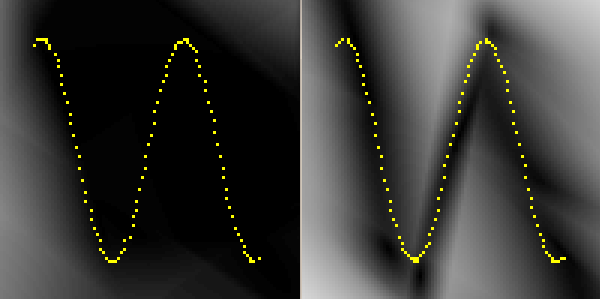
\includegraphics[scale=0.25]{./figures/SATAE/toy_shrink.png}
\caption{Energy surfaces for unregularized (left), and regularized (right)
solutions obtained on SATAE-shrink and 10 basis vectors. Black corresponds to
low reconstruction energy. Training points lie on a one-dimensional manifold
shown in yellow.}  \label{fig:toyshrink} \end{figure} 

\begin{figure} \centering
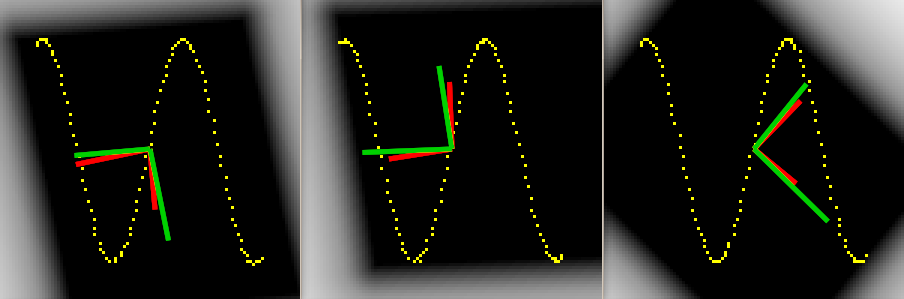
\includegraphics[scale=0.25]{./figures/SATAE/toy_sat_linear_noreg.png}
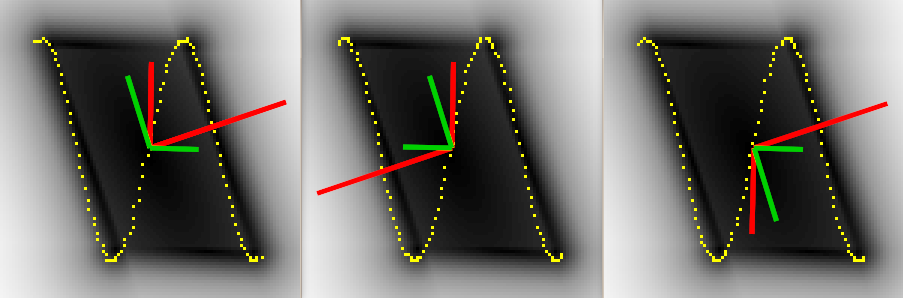
\includegraphics[scale=0.25]{./figures/SATAE/toy_sat_linear_reg.png} \caption{SATAE-SL toy
example with two basis elements. Top Row: three randomly initialized solutions
obtained with no regularization. Bottom Row: three randomly initialized
solutions obtained with regularization.}  \label{fig:toysatlinear} \end{figure} 

Note that $shrink_c(W^e x + b^e) =  abs(shrink(W^e x + b^e))$, which
corresponds to an $L_1$ penalty on the activations. Thus this SATAE is
equivalent to a sparse auto-encoder with a shrink activation function. Given
the equivalence to the sparse auto-encoder we anticipate the same scale
ambiguity which occurs with $L_1$ regularization. This ambiguity can be avoided
by normalizing the decoder weights to unit norm. It is expected that the
SATAE-shrink will learn similar features to those obtained with a sparse
auto-encoder, and indeed this is what we observe. Figure~\ref{fig:results}(c)
shows the decoder filters learned by an auto-encoder with shrink nonlinearity
trained on gray-scale natural image patches. One can recognize the expected
Gabor-like features when the saturation penalty is activated. When trained on
the binary MNIST dataset the learned basis is comprised of portions of digits
and strokes. Nearly identical results are obtained with a SATAE which uses a
rectified-linear activation function. This is because a rectified-linear
function with an encoding bias behaves as a positive only shrink function,
similarly the complementary function is equivalent to a positive only $L_1$
penalty on the activations.          

\newcommand\x{2.5cm}
\newcommand\y{8cm} 

\afterpage{
%\clearpage
\thispagestyle{empty}
\begin{figure} 
\centering \begin{subfigure}[b]{0.225\textwidth} \centering
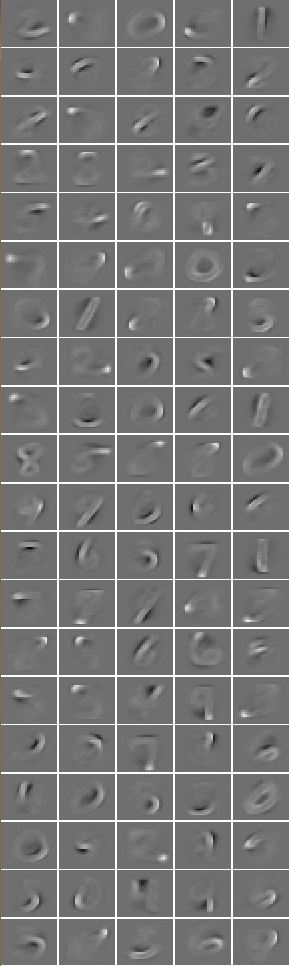
\includegraphics[width=\x, height=\y]{./figures/SATAE/strokes_full.png} \caption{}
\end{subfigure} \begin{subfigure}[b]{0.225\textwidth} \centering
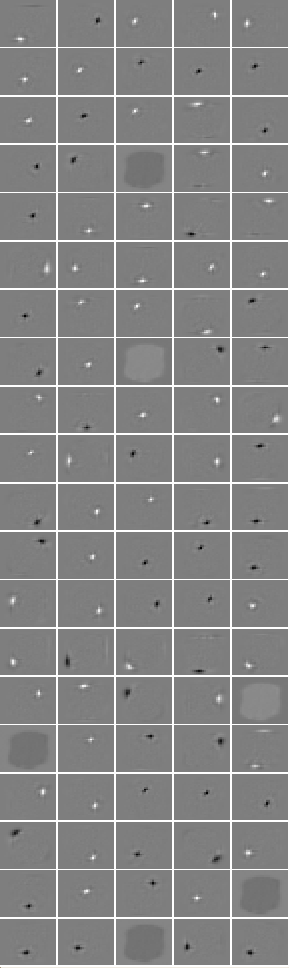
\includegraphics[width=\x, height=\y]{./figures/SATAE/MNIST_sat_linear_full.png}
\caption{} \end{subfigure} \begin{subfigure}[b]{0.2\textwidth} \centering
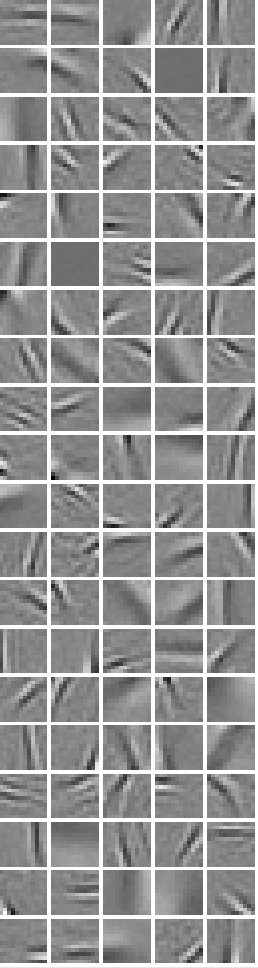
\includegraphics[width=\x, height=\y]{./figures/SATAE/gabors_full.png} \caption{}
\end{subfigure} \begin{subfigure}[b]{0.2\textwidth} \centering
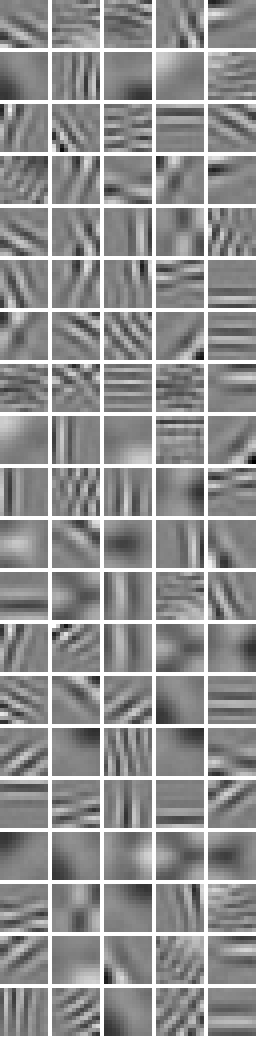
\includegraphics[width=\x, height=\y]{./figures/SATAE/patches_sat_linear_full.png}
\caption{} \end{subfigure} \\ \begin{subfigure}[b]{0.225\textwidth} \centering
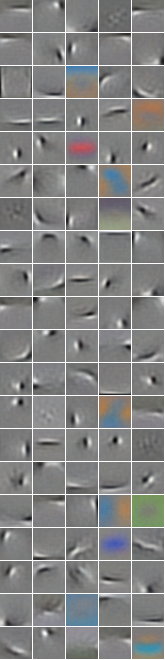
\includegraphics[width=\x, height=\y]{./figures/SATAE/CIFAR_shrink01.png} \caption{}
\end{subfigure} \begin{subfigure}[b]{0.225\textwidth} \centering
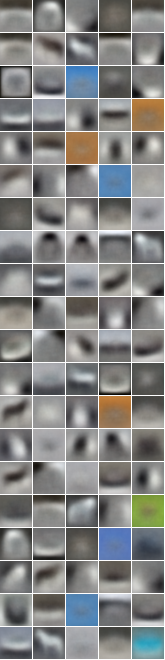
\includegraphics[width=\x, height=\y]{./figures/SATAE/CIFAR_shrink05.png} \caption{}
\end{subfigure} \begin{subfigure}[b]{0.2\textwidth} \centering
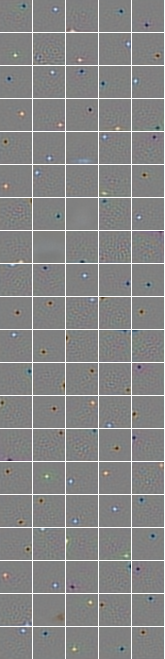
\includegraphics[width=\x, height=\y]{./figures/SATAE/CIFAR_sat_linear300_1.png}
\caption{} \end{subfigure} \begin{subfigure}[b]{0.2\textwidth} \centering
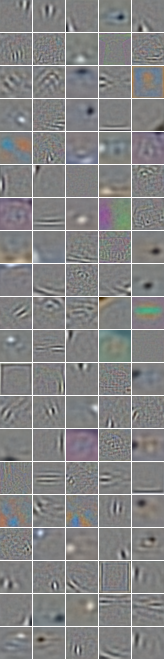
\includegraphics[width=\x, height=\y]{./figures/SATAE/CIFAR_sat_linear300_6.png}
\caption{} \end{subfigure} \caption{\small Basis elements learned by the SATAE using
different nonlinearities on: 28x28 binary MNIST digits, 12x12 gray scale
natural image patches, and CIFAR-10. (a) SATAE-shrink trained on MNIST, (b)
SATAE-saturated-linear trained on MNIST, (c) SATAE-shrink trained on natural
image patches, (d) SATAE-saturated-linear trained on natural image patches,
(e)-(f) SATAE-shrink trained on CIFAR-10 with $\alpha=0.1$ and $\alpha=0.5$,
respectively, (g)-(h) SATAE-SL trained on CIFAR-10 with $\alpha=0.1$ and
$\alpha=0.6$, respectively.  } \label{fig:results} \end{figure}
\clearpage} 

\begin{figure} \centering 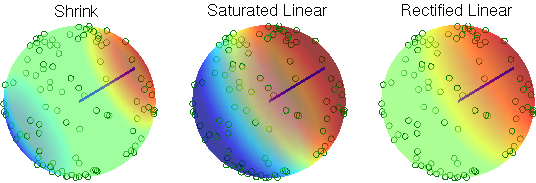
\includegraphics[scale=0.5]{./figures/SATAE/viz_nonlin.png}
\caption{Geometric visualization of non-linearities}
\end{figure} 


\begin{figure} \centering \begin{subfigure}[b]{0.15\textwidth} \centering
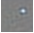
\includegraphics[scale=2]{./figures/SATAE/1.png}\\ 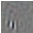
\includegraphics[scale=2]{./figures/SATAE/horse1.png} 
        %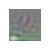
\includegraphics[scale=2]{.//objects/red/0.png} \\
        %\caption{$\alpha=0$}
    \end{subfigure} \begin{subfigure}[b]{0.15\textwidth} \centering
    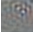
\includegraphics[scale=2]{./figures/SATAE/2.png} \\
    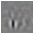
\includegraphics[scale=2]{./figures/SATAE/horse2.png} 
        %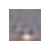
\includegraphics[scale=2]{.//objects/red/1.png} \\
        %\caption{$\alpha=0.1$}
    \end{subfigure} \begin{subfigure}[b]{0.15\textwidth} \centering
    
\includegraphics[scale=2]{./figures/SATAE/3.png}\\
    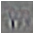
\includegraphics[scale=2]{./figures/SATAE/horse3.png} 
        %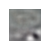
\includegraphics[scale=2]{.//objects/red/2.png} \\
		
        %\caption{$\alpha=0.2$}
    \end{subfigure} \begin{subfigure}[b]{0.15\textwidth} \centering
    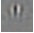
\includegraphics[scale=2]{./figures/SATAE/4.png} \\
    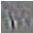
\includegraphics[scale=2]{./figures/SATAE/horse4.png} 
        %
\includegraphics[scale=2]{.//objects/red/3.png} \\
        %\caption{$\alpha=0.5$}
    \end{subfigure} \begin{subfigure}[b]{0.15\textwidth} \centering
    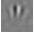
\includegraphics[scale=2]{./figures/SATAE/5.png} 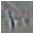
\includegraphics[scale=2]{./figures/SATAE/horse5.png}
    \\
        %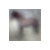
\includegraphics[scale=2]{./objects/red/4.png} \\
		
        %\caption{$\alpha=1$} 
    \end{subfigure} \caption{Evolution of two filters with increasing
    saturation regularization for a SATAE-SL trained on CIFAR-10. Filters
    corresponding to larger values of $\alpha$ were initialized using the
    filter corresponding to the previous $\alpha$. The regularization parameter
    was varied from 0.1 to 0.5 (left to right) in the top five images and 0.5
    to 1 in the bottom five } \label{fig:horse} \end{figure} 

\subsection{SATAE-saturated-linear} Unlike the SATAE-shrink, which tries to
compress the data by minimizing the number of active elements; the SATAE
saturated-linear (SATAE-SL) tries to compress the data by encouraging the
latent code to be as close to binary as possible. Without a saturation penalty
this auto-encoder learns to encode small groups of neighboring pixels. More
precisely, the auto-encoder learns the identity function on all datasets. An
example of such a basis is shown in Figure \ref{fig:results}(b). With this
basis the auto-encoder can perfectly reconstruct any input by producing small
activations which stay within the linear region of the nonlinearity.
Introducing the saturation penalty does not have any effect when training on
binary MNIST. This is because the scaled identity basis is a global minimizer
of Equation 2 for the SATAE-SL on any binary dataset. Such a basis can
perfectly reconstruct any binary input while operating exclusively in the
saturated regions of the activation function, thus incurring no saturation
penalty. On the other hand, introducing the saturation penalty when training on
natural image patches induces the SATAE-SL to learn a more varied basis (Figure
\ref{fig:results}(d)). 

\subsection{Experiments on CIFAR-10} SATAE auto-encoders with 100 and 300 basis
elements were trained on the CIFAR-10 dataset, which contains small color
images of objects from ten categories. In all of our experiments the
auto-encoders were trained by progressively increasing the saturation penalty
(details are provided in the next section). This allowed us to visually track
the effect of the saturation penalty on individual basis elements. Figure
\ref{fig:results}(e)-(f) shows the basis learned by SATAE-shrink with small and
large saturation penalty, respectively. Increasing the saturation penalty has
the expected effect of reducing the number of nonzero activations. As the
saturation penalty increases, active basis elements become responsible for
reconstructing a larger portion of the input. This induces the basis elements
to become less spatially localized. This effect can be seen by comparing
corresponding filters in Figure \ref{fig:results}(e) and (f). Figures
\ref{fig:results}(g)-(h)  show the basis elements learned by SATAE-SL with
small and large saturation penalty, respectively. The basis learned by SATAE-SL
with a small saturation penalty resembles the identity basis, as expected (see
previous subsection). Once the saturation penalty is increased small
activations become more heavily penalized. To increase their activations the
encoding basis elements may increase in magnitude or align themselves with the
input. However, if the encoding and decoding weights are tied (or fixed in
magnitude) then reconstruction error would increase if the weights were merely
scaled up. Thus the basis elements are forced to align with the data in a way
that also facilitates reconstruction. This effect is illustrated in Figure
\ref{fig:horse} where filters corresponding to progressively larger values of
the regularization parameter are shown. The top half of the figure shows how an
element from the identity basis ($\alpha=0.1$) transforms to a localized edge
($\alpha=0.5$). The bottom half of the figure shows how a localized edge
($\alpha=0.5$) progressively transforms to a template of a horse ($\alpha=1$).

\section{Experimental Details} Because the regularizer explicitly encourages
activations in the zero gradient regime of the nonlinearity, many encoder basis
elements would not be updated via back-propagation through the nonlinearity if
the saturation penalty were large. In order to allow the basis elements to
deviate from their initial random states we found it necessary to progressively
increase the saturation penalty. In our experiments the weights obtained at a
minimum of Equation 2 for a smaller value of $\alpha$ were used to initialize
the optimization for a larger value of $\alpha$. Typically, the optimization
began with $\alpha=0$ and was progressively increased to $\alpha=1$ in steps of
$0.1$. The auto-encoder was trained for 30 epochs at each value of $\alpha$.
This approach also allowed us to track the evolution of basis elements as a
function of $\alpha$ (Figure \ref{fig:horse}). In all experiments data samples
were normalized by subtracting the mean and dividing by the standard deviation
of the dataset. The auto-encoders used to obtain the results shown in Figure
\ref{fig:results} (a),(c)-(f) used 100 basis elements, others used 300 basis
elements. Increasing the number of elements in the basis did not have a strong
qualitative effect except to make the features represented by the basis more
localized. The decoder basis elements of the SATAEs with shrink and
rectified-linear nonlinearities were reprojected to the unit sphere after every
10 stochastic gradient updates. The SATAEs which used saturated-linear
activation function were trained with tied weights.  All results presented were
obtained using stochastic gradient descent with a constant learning rate of
0.05.

\section{Discussion}

In this work we have introduced a general and conceptually simple latent state
regularizer. It was demonstrated that a variety of feature sets can be obtained
using a single framework. The utility of these features depend on the
application. In this section we extend the definition of the saturation
regularizer to include functions without a zero-gradient region. The
relationship of SATAEs with other regularized auto-encoders will be discussed.
We conclude with a discussion on future work.   

\subsection{Extension to Differentiable Functions} We would like to extend the
saturation penalty definition (Equation 1) to differentiable functions without
a zero-gradient region. An appealing first guess for the complimentary function
is some positive function of the first derivative, $f_c(x) = |f'(x)|$ for
instance. This may be an appropriate choice for monotonic activation functions
which have their lowest gradient regions at the extrema (e.g. sigmoids).
However some activation functions may contain regions of small or zero gradient
which have negligible extent, at the extrema for instance. We would like our
definition of the complimentary function to not only measure the local gradient
in some region, but to also measure it's extent. For this purpose we employ the
concept of average variation over a finite interval. We define the average
variation of $f$ at $x$ in the positive and negative directions at scale $l$,
respectively as: 

\begin{eqnarray} \nonumber \Delta_l^+ f(x) &=& \frac{1}{l} \int_x ^{x+l}
|f'(u)| du = |f'(x)| * \Pi_l^+(x)\\ \nonumber \Delta_l^- f(x) &=& \frac{1}{l}
\int_{x-l} ^x |f'(u)| du = |f'(x)| * \Pi_l^-(x).  \end{eqnarray} 

Where $*$ denotes the continuous convolution operator. $\Pi_l^+(x)$ and
$\Pi_l^-(x)$ are uniform averaging kernels in the positive and negative
directions, respectively. Next, define a directional measure of variation of
$f$ by integrating the average variation at all scales. 

\begin{eqnarray} \nonumber M^+ f(x) &=& \int_0^{+\infty} \Delta_l^+ f(x) w(l)dl
= \left[\int_0^{+\infty} w(l) \Pi^+_l(x) dl \right] * |f'(x)| \\ \nonumber M^-
f(x) &=& \int_0^{+\infty} \Delta_l^- f(x) w(l)dl = \left[\int_0^{+\infty} w(l)
\Pi^-_l(x) dl \right] * |f'(x)| .  \end{eqnarray} 

Where $w(l)$ is chosen to be a sufficiently fast decreasing function of $l$ to
insure convergence of the integral. The integral with which $|f'(x)|$ is
convolved in the above equation evaluates to some decreasing function of $x$
for $\Pi^+$ with support $x \geq 0$. Similarly, the integral involving $\Pi^-$
evaluates to some increasing function of $x$ with support $x \leq 0$. This
function will depend on $w(l)$. The functions $M^+f(x)$ and $M^-f(x)$ measure
the average variation of $f(x)$ at all scales $l$ in the positive and negative
direction, respectively. We define the complimentary function $f_c(x)$ as: 

\begin{equation} f_c(x) = min(M^+f(x),M^-f(x)).  \end{equation} 

\begin{figure} \centering 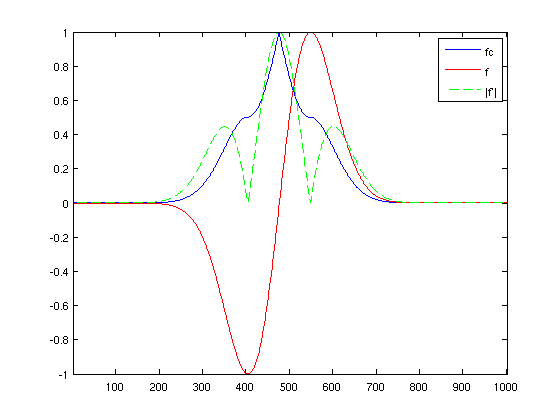
\includegraphics[scale=0.43]{./figures/SATAE/diff_cc.png}
\caption{Illustration of the complimentary function ($f_c$) as defined by
Equation 3 for a non-monotonic activation function ($f$). The absolute
derivative of $f$ is shown for comparison.}  \label{fig:diff_cc} \end{figure} 

An example of a complimentary function defined using the above formulation is
shown in Figure~\ref{fig:diff_cc}. Whereas $|f'(x)|$ is minimized at the
extrema of $f$, the complimentary function only plateaus at these locations.

\subsection{Relationship with the Contractive Auto-Encoder} Let $h_i$ be the
output of the $i^{th}$ hidden unit of a single-layer auto-encoder with
point-wise nonlinearity $f(\cdot)$. The regularizer imposed by the contractive
auto-encoder (CAE) can be expressed as follows: 

\begin{equation} \nonumber \sum_{ij} \left(\frac{\partial h_i}{\partial x_j}
\right)^2 = \sum_i ^{d_h} \left(f'(\sum_{j=1}^d W^e_{ij}x_j + b_i)^2 \| W^e_i
\| ^2 \right), \end{equation}  
 
\noindent where $x$ is a $d$-dimensional data vector, $f'(\cdot)$ is the
derivative of $f(\cdot)$, $b_i$ is the bias of the $i^{th}$ encoding unit, and
$W^e_i$ denotes the $i^{th}$ row of the encoding weight matrix. The first term
in the above equation tries to adjust the weights so as to push the activations
into the low gradient (saturation) regime of the nonlinearity, but is only
defined for differentiable activation functions. Therefore the CAE indirectly
encourages operation in the saturation regime. Computing the Jacobian, however,
can be cumbersome for deep networks. Furthermore, the complexity of computing
the Jacobian is $O(d \times d_h)$, although a more efficient implementation is
possible \cite{CAE}, compared to the $O(d_h)$ for the saturation penalty.  
 
\subsection{Relationship with the Sparse Auto-Encoder} In Section 3.2 it was
shown that SATAEs with shrink or rectified-linear activation functions are
equivalent to a sparse auto-encoder. Interestingly, the fact that the
saturation penalty happens to correspond to $L_1$ regularization in the case of
SATAE-shrink agrees with the findings in \cite{LISTA}. In their efforts to find
an architecture to approximate inference in sparse coding, Gregor et al. found
that the shrink function is particularly compatible with $L_1$ minimization.
Equivalence to sparsity only for some activation functions suggests that SATAEs
are a generalization of sparse auto-encoders. Like the sparsity penalty, the
saturation penalty can be applied at any point in a deep network for the same
computational cost. However, unlike the sparsity penalty the saturation penalty
is adapted to the nonlinearity of the particular layer to which it is applied. 

\chapter{Convolutional Sparse Inference}
\label{chapter:LISTA} 
\chapter{Learning Spatiotemporally Coherent Metrics}
\label{chapter:slow} 
\chapter{Learning to Linearize under Uncertainty}
\label{chapter:error} 
\chapter{Adversarial Inpainting}
\label{chapter:uncertainty}
\chapter{Conclusion} 
\label{chapter:conclusion} 

\FloatBarrier
\clearpage

\addtocontents{toc}{\protect\setcounter{tocdepth}{+1}}
\addcontentsline{toc}{chapter}{Conclusions}
\section*{Conclusions}
%We have shown that discriminative ConvNet architectures are able to accurately and efficiently estimate the pose of humans in images. While it is not clear if one architecture is applicable to all problem domains, we have never-the-less shown that networks adapted to the problem are able to out-perform existing methods via \emph{domain-specific optimizations}. We have demonstrated such optimizations on two example problem domains:  1) monocular hand-pose recognition from depth images and 2) monocular full body-pose recognition from RGB images.

In Part~\ref{part:one} we presented a novel pipeline for tracking the instantaneous pose of articulable objects from a single depth image. As an application of this pipeline we showed state-of-the-art results for tracking human hands in real-time using commodity hardware. This pipeline leverages the accuracy of offline model-based dataset generation routines in support of a robust real-time ConvNet architecture for feature extraction. We showed that it is possible to use intermediate heat-map features to extract accurate and reliable 3D pose information at interactive frame-rates using inverse kinematics. To build the ConvNet architecture we applied domain-specific applications related to the human hand and since it is possible to use the output of the RDF stage to crop, center and scale the incoming depth image around the hand, we showed that it is possible to use a large fully-connected layer in the network architecture without significant overtraining (since translation invariance need not be learned).

Building upon the results from Part~\ref{part:one}, in Parts~\ref{part:two}, \ref{part:three} and \ref{part:four} we applied an adapted sliding-window based ConvNet architecture to the problem of full-body tracking in monocular RGB images.  For this application we did not have access to a depth image source, however we were able to incorporate connectivity priors to improve the ConvNet architecture as a domain-specific optimization. This was achieved via a novel ConvNet Part-Detector and an MRF inspired Spatial-Model which can be efficiently incorporated into a single learning framework. This new network paradigm significantly outperforms existing architectures on the task of human body pose recognition.  Training and inference of our architecture uses commodity level hardware and runs at close to real-time frame rates, making this technique tractable for a wide variety of application areas.  For future work we expect to further improve upon these results by increasing the complexity and expressiveness of our simple spatial model (especially for unconstrained datasets like LSP and MPII).

In Part~\ref{part:three} we showed that when incorporating both RGB and motion features in our deep ConvNet architecture, our network is able to outperform existing state-of-the-art techniques for the task of human body pose detection in video and improve upon the baseline model of Part~\ref{part:two}. We have also shown that using motion features alone can outperform some traditional algorithms~\cite{Eichner:2009:BAM, yang11cvpr, sapp11eccv}. Our findings suggest that even very simple temporal cues can greatly improve performance with a very minor increase in model complexity. As such, we suggest that future work should place more emphasis on the correct use of motion features.  We would also like to further explore higher level temporal features, potentially via learned spatiotemporal convolution stages and we hope that using a more expressive temporal-spatial model (using motion constraints) will help improve performance significantly.

Though originally developed for the task of classification~\cite{LeCunMNIST}, deep ConvNets have been successfully applied to a multitude of other problems. In classification all variability except the object identity is suppressed. On the other hand, localization tasks such as human body pose estimation often demand a high degree of spatial precision. In Part~\ref{part:four} we presented a domain-specific optimization that is able to efficiently recover the precision lost due to pooling in traditional ConvNet architectures while maintaining the computational benefits of pooling with decimation (or downsampling). We presented a novel cascaded architecture that combined fine and coarse scale convolutional networks, to achieve new state-of-the-art results on the FLIC~\cite{modec} and MPII-human-pose\cite{andriluka14cvpr} datasets.


%\begin{appendices}
%\addtocontents{toc}{\protect\setcounter{tocdepth}{-1}}
%\appendixchapter{TODO}
%% Appendix goes here
%\end{appendices}

\FloatBarrier
\newpage

%\addtocontents{toc}{\protect\setcounter{tocdepth}{+1}}
\addcontentsline{toc}{chapter}{Bibliography}

\singlespacing
\printbibliography
\end{document}
